\documentclass[12pt]{report}
\usepackage[utf8]{inputenc}
\usepackage{a4}
\usepackage[none]{hyphenat} %hyphenation
\sloppy
\usepackage{parskip} %no indentation after paragraphs
\usepackage{umlaute}
\usepackage{listings}
\usepackage{afterpage} %for using \afterpage{\clearpage} (don't push images to the end of a chapter)
\usepackage{makeidx}
\usepackage[numbers]{natbib}
\usepackage{graphicx}
\usepackage{picins} %provides precise control over the placement of inline graphics
\usepackage{setspace}
\usepackage{titlesec}
\usepackage{dsfont} %math symbols
\usepackage{tabularx}
\usepackage{floatflt} %float text around figures and tables
% Florian Schulze, 06.06.2012
% v1.0, latest edit: 06.06.2012

\usepackage{enumitem} %resume counting from previous enumerate block
\usepackage{amsmath,amssymb}
\usepackage[format=default,font=footnotesize,labelfont=bf]{caption}
\usepackage{listings} %for listing source code
\usepackage{color}
\usepackage{algpseudocode} %for listing pseudocode
\usepackage{algorithm} %wrap algpseudocode and enrich with label etc.
\usepackage{float} % for [H] after floats

\titleformat{\paragraph}[hang]{\normalfont\bfseries}{\theparagraph}{.5em}{}

\makeindex
\frenchspacing
\sloppy

\pagestyle{headings}

\textwidth16cm
\textheight22cm

\topmargin0cm
\oddsidemargin0cm
\evensidemargin0cm


\newcommand{\bildklein}[3]{  
	\begin{figure}[hp]
	\begin{center}
	\includegraphics[width=0.5\textwidth]{#1}
	\end{center}
	\caption[#2]{#3}
	\end{figure}
}
  	
\newcommand{\bildgross}[3]{  
	\begin{figure}[hp]
	\begin{center}
	\includegraphics[width=0.95\textwidth]{#1}
	\end{center}
	\caption[#2]{#3}
	\end{figure}
}
  

\newcommand{\eqn}[3]{
	\begin{figure}[hp]
	\begin{equation}#1\end{equation}
	\caption[#2]{#3}
	\end{figure}
}

% This is tumlogo.tex
%
% Neues TUM-Logo in TeX
%   by G. Teege, 19.10.89
% Benutzung:
%   Am Anfang des Dokuments (TeX oder LaTeX):
%     \input tumlogo
%   Dann beliebig oft:
%     \TUM{<breite>}
%   bzw.
%     \oTUM{<breite>}
%   \TUM setzt das Logo mit der Breite <breite> und der entsprechenden Hoehe.
%   <breite> muss eine <dimen> sein. \oTUM erzeugt eine "outline"-Version
%   des Logos, d.h. weiss mit schwarzem Rand. Bei \TUM ist es ganz schwarz.
%   \oTUM entspricht damit der offiziellen Version des Logos.
%   Das Logo kann wie ein einzelnes Zeichen verwendet werden.
%   Beispiel:
%     Dies ist das TUM-Logo: \oTUM{1cm}.
%
\def\TUM#1{%
\dimen1=#1\dimen1=.1143\dimen1%
\dimen2=#1\dimen2=.419\dimen2%
\dimen3=#1\dimen3=.0857\dimen3%
\dimen4=\dimen1\advance\dimen4 by\dimen2%
\setbox0=\vbox{\hrule width\dimen3 height\dimen1 depth0pt\vskip\dimen2}%
\setbox1=\vbox{\hrule width\dimen1 height\dimen4 depth0pt}%
\setbox2=\vbox{\hrule width\dimen3 height\dimen1 depth0pt}%
\setbox3=\hbox{\copy0\copy1\copy0\copy1\box2\copy1\copy0\copy1\box0\box1}%
\leavevmode\vbox{\box3}}
%
\def\oTUM#1{%
\dimen1=#1\dimen1=.1143\dimen1%
\dimen2=#1\dimen2=.419\dimen2%
\dimen3=#1\dimen3=.0857\dimen3%
\dimen0=#1\dimen0=.018\dimen0%
\dimen4=\dimen1\advance\dimen4 by-\dimen0%
\setbox1=\vbox{\hrule width\dimen0 height\dimen4 depth0pt}%
\advance\dimen4 by\dimen2%
\setbox8=\vbox{\hrule width\dimen0 height\dimen4 depth0pt}%
\advance\dimen4 by-\dimen2\advance\dimen4 by-\dimen0%
\setbox4=\vbox{\hrule width\dimen4 height\dimen0 depth0pt}%
\advance\dimen4 by\dimen1\advance\dimen4 by\dimen3%
\setbox6=\vbox{\hrule width\dimen4 height\dimen0 depth0pt}%
\advance\dimen4 by\dimen3\advance\dimen4 by\dimen0%
\setbox9=\vbox{\hrule width\dimen4 height\dimen0 depth0pt}%
\advance\dimen4 by\dimen1%
\setbox7=\vbox{\hrule width\dimen4 height\dimen0 depth0pt}%
\dimen4=\dimen3%
\setbox5=\vbox{\hrule width\dimen4 height\dimen0 depth0pt}%
\advance\dimen4 by-\dimen0%
\setbox2=\vbox{\hrule width\dimen4 height\dimen0 depth0pt}%
\dimen4=\dimen2\advance\dimen4 by\dimen0%
\setbox3=\vbox{\hrule width\dimen0 height\dimen4 depth0pt}%
\setbox0=\vbox{\hbox{\box9\lower\dimen2\copy3\lower\dimen2\copy5%
\lower\dimen2\copy3\box7}\kern-\dimen2\nointerlineskip%
\hbox{\raise\dimen2\box1\raise\dimen2\box2\copy3\copy4\copy3%
\raise\dimen2\copy5\copy3\box6\copy3\raise\dimen2\copy5\copy3\copy4\copy3%
\raise\dimen2\box5\box3\box4\box8}}%
\leavevmode\box0}
% End of tumlogo.tex



\begin{document}

\nocite{*} %include uncited references in bibliography
\hoffset=5mm
\thispagestyle{empty}

\begin{center}
	\bigskip \bigskip \bigskip 
	\oTUM{6.0cm} \\
	\vspace*{0.8cm}
	{\huge \bf Technische Universität} \\
	\bigskip
	{\huge \bf München} \\
	\bigskip \bigskip \bigskip
	{\huge \bf Fakultät für Informatik} \\
	\bigskip \bigskip \bigskip
	{\Large \bf Bachelor's Thesis in Informatik} \\
	\bigskip \bigskip \bigskip \bigskip \bigskip
	{\Large The housing market under a supply shortage} \\        
	\bigskip \bigskip \bigskip \bigskip
	{\Large Ricardo Sebastian Vera Jacob} \\    
	\bigskip
	\begin{figure}[ht]
	\centering 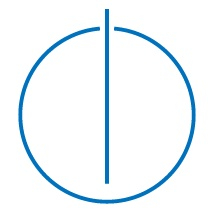
\includegraphics[width=0.2\linewidth]{figures/infologo.jpg}
	\end{figure}
	\bigskip 
\end{center}

\vfill

\newpage
\hoffset=5mm
\thispagestyle{empty}

\begin{center}
	\bigskip \bigskip \bigskip 
	\oTUM{6.0cm} \\
	\vspace*{0.8cm}
	{\huge \bf Technical University of} \\
	\bigskip
	{\huge \bf Munich} \\
	\bigskip \bigskip \bigskip
	{\huge \bf Department of Informatics} \\
	\bigskip \bigskip \bigskip
	{\Large \bf Bachelor's Thesis in Informatics} \\
	\bigskip \bigskip \bigskip \bigskip \bigskip
	{\Large The housing market under a supply shortages} \\
	\bigskip \bigskip \bigskip
	{\Large Der Wohnungsmarkt in einer Angebotsknappheit.} \\
	\bigskip
\end{center}
\vfill

\begin{tabular}{ll}
{\Large \bf Author:} & {\Large Ricardo Sebastian Vera Jacob} \\\\
{\Large \bf Supervisor:} & {\Large Prof. Dr. Martin Bichler} \\\\
{\Large \bf Advisor:} & {\Large Donghao Zhu} \\\\
{\Large \bf Submission:} & {\Large 28.02.2022}
\end{tabular}

\newpage	
\thispagestyle{empty}
\hoffset=0mm
\vspace*{\fill}
\noindent I assure the single handed composition of this master's thesis only supported by declared resources.\\\\
Munich, 28.02.2022\\\\\\\\\\\\
\noindent \textit{(Ricardo Sebastian Vera Jacob)}

\newpage
\thispagestyle{empty}
\null

\newpage
\thispagestyle{empty}
\hoffset=0mm
\section*{Abstract}	
\begin{spacing}{1.2}
This paper modeled the housing market by splitting it into three subcategories. Then on this model model compute simulations of it and lastly discus the results. The market will be divided from the supply side as follows: category one for subsidised public allocation (that will match agents with a FCFS queue), social advertised that includes all allocation that can be found publicly (as in web sites or social media), agents will have a probability to be matched to an apartment here and lately decide to take it or not and lastly accommodation found trough the help of landlord or real estate agency, agents will choose this category at last. Moreover the agents will have a maximum waiting time to find accommodation and after that they will perish and leave the market. Lastly the arrivals of houses and agents will be modeled with the help of Poisson processes. After the simulations were done we were able to observe that agents highly favorites the public subsidised sector. Another import point to remark is that the model showed that the system can reach an equilibrium where all agents have an apartment matched to them. However for that there should be more apartments available in the market than demand, otherwise agents will leave the market. Agents will leave the market even with a balanced market where there is exactly one apartment for each agent and exactly one agent for each apartment. Moreover we provided an open source code in order to further research and expand the model to fit to the desired needs.
\end{spacing}

\newpage
\setcounter{page}{1}
\hoffset=0mm
\bibliographystyle{wmaainf} % quotation style
\setcounter{tocdepth}{3}
\setcounter{secnumdepth}{3}
\fboxsep 0mm

\tableofcontents

\newpage
\setlength{\baselineskip}{3ex}

\begin{spacing}{1.15}
	\chapter{Introduction}
This paper will examine the supply-demand chain in the housing market with an inclination towards high demand and low supply. Some great examples of these type of markets are: Vienna, Munich, New York or London among others. Where the demand for apartments is significantly higher than the actual market supply and chances of finding accommodation at a fair price at said locations are often very slim or non existent. With citizens usually having to take the first and often only offer they get for accommodation. This can cause an inefficient distribution of residences across the city or even having to search for accommodation in the suburbs and leaving the city housing market causing long commutes and wasted time. The purpose of this paper is to understand the current situation of the over saturation of the market better. 
Specifically we will focus our attention to the allocation of residences under the adoption of the approaches a citizen has to find accommodation. From using a private real estate agent to getting a social subsidised residence. With the isolation of the market into several categories, we can then observe how and where agents find accommodation and thus examine the distribution and behaviour of the system. Then we can define the key variables that cause such distributions and from there observe the behaviour under changing factors.

Moreover with the help of this model, literature and simulations we will be able to observe the behaviour of the system, draw conclusion and alter the model variables in order to simulate other situations of the market as changes in the supply-demand chain. From now on instead of referring to people, landlords or citizens we will refer to them as agents. This will avoid confusion and redundancy. We will develop a model that emulates the market as close as possible with the help of probabilistic tools as poison processes and exponential distributions, to design the arrival and exit of agents in the market and implement an algorithm for the assigning of residences to the agents. 

An agent is defined as an entity that entered the market with the goal of finding accommodation and stay in the current market. In order to achieve that the agent counts with several variables and data structures. First he has a maximum waiting time. This time is calculated by a exponential distribution
\begin{equation} \label{eq1}
{\displaystyle \operatorname {E} [X]={\frac {1}{\lambda}}}
\end{equation} 
Where $\lambda$ represents the average waiting time. The agent has said time to find accommodation and if he runs out of it he "perishes" and has to leave the market without success. In this case we can define $\lambda$ as 10 to simplify the model. An agent also has a list of all matched apartments that he can consult at any time and from those choose to take one. With these set of variables he can now enter the market, but first we have to define how the market works and how it is divided.

To approximate the model as close as possible to reality we will define three categories in which agents can actively search for accommodation:
\begin{itemize}
        \item \textbf{Category 1}: government non-profit subsidised organizations as "Studentenwerk" in Germany that offer cheap alternatives but long waiting times. Low supply and very high demands, with waiting times ranging from one to three years but in the end this is the category where agents maximise their utility (cheapest option)
        \item \textbf{Category 2}: free advertising platforms such as immocheck24, Facebook groups, wg-gesucht or newspapers and any other form of direct contact landlord-agent are enclosed into this category. This alternative offer a direct contact from the landlords to the tenants. With the assumption that this is by far the most common used platform to find accommodation.
        \item \textbf{Category 3}: real estate agents that are usually the most expensive option but often the one with highest chances of success. With lower demand but higher (pricier) supply.
\end{itemize}

Additionally each of these categories has a set of variables and independent matching system that in the end form the supply pool of apartments. For this we will define their variables and matching conditions. Next we will describe their working structure starting with category 1.

For a agent to get public accommodation certain criteria has to be fulfilled. First the agent has to be actively searching for accommodation and still have time until he has to leave the market. Then he enters a first come first served (FCFS) queue with other agents and has to wait until a house is matched to him. This process can only assign accommodation to the agents if there are enough available supply of apartments and when new apartments join the market. We can deduce that the probability \textbf{pMC1} of getting \textbf{M}atched to an apartment depends on the length of the queue and the supply of the market. In that case the agent in the first position of the queue gets the apartment matched to him, then the agent has a probability \textbf{pTC1} of \textbf{T}aking said apartment. If the agent doesn't take said apartment he goes back to the queue and has to wait again until another opportunity arises.

On the other hand if an agent wants to enter the social housing market or category 2 the process changes. Here the searching agent applies for all available apartments and has a probability \textbf{pMC2} of being successfully matched to said apartment. Since it is of self interest of the agent to get accommodation firstly in category 1 (since as mentioned in the description of the categories this option offers a higher utility for the agent) it will wait until he has no time left before he has to leave the market. At the time he has to leave the market he will then search in the apartments he got matched to in category 2 and then choose one that is still available. If there are no available apartments the agent leaves the market. If there is an apartment available he has the probability \textbf{pTC2} of taking the apartment. This probability depends on the supply of apartments in the market and the demand.

The last category is used by agents only when they are about to perish and are desperate for accommodation and couldn't find an apartment by any means. They would apply to the market with matching probability \textbf{pMC3}. Here The probability of being matched is the highest in the market but the probability of taking said apartment is the lowest \textbf{pTC3}. They would have the choice of taking the accommodation with a lower probability than in Category 1 (C1) and in Category 2 (C2) but the matching probability is higher. 

Hence we can assume a set of  axioms to further specify the market. The matching probability in the market is defined as:
\begin{equation} \label{eq2}
pMC1 \subset pMC2 \subset pMC3.
\end{equation} 
The lower the category the less probable is to get matched to an apartment. For the probability of taking said matched apartment is defined as:
\begin{equation} \label{eq3}
pTC3 \subset pTC2 \subset pTC1.
\end{equation}
Where the agent would almost immediately take accommodation in the public endorsed sector. In this case the lower the category the most likely it is for the agent to take the matched apartment. Lastly for the cardinality of the supply of apartments in each category will be defined as follows:
\begin{equation} \label{eq4}
C1 \subset C3 \subset C2.
\end{equation}
Here the category with highest supply is C2 with C1 being the one with the lowest supply.

Now we have to define the way in which agents arrive to the market. The housing market is a highly fluctuating market, with agents coming and leaving. The same can be said for the apartments with the exception that the probability of a new apartment coming to the market is lower. For this purpose we will model the arrival of agents/apartments with the help of a poison process. 
\begin{equation} \label{eq5}
P(t, \lambda) = \frac{\lambda^t e^{-\lambda}}{t!} 
\end{equation}
For this, t represents the time units and $\lambda$ the mean average. Since time is equal for the market the only variable we can modify for each category is $\lambda$. Since described in the formula \ref{eq4} the lambdas can be derived from the cardinality of the categories. With the following equation:
\begin{equation} \label{eq6}
\lambda C1 \subset \lambda C3 \subset \lambda C2
\end{equation}

This way we ensure that at every point in time the cardinality of the groups is maintained. In this model the supply side of the market is divided but the demand side is shared across the different categories so for the modeling of the arrival of the agents we only need one variable, thus being $\lambda$A. For this with the help of the last equation we can expand it to include the arrival of the agents and assume that there is always more or equal demand than there is supply:
\begin{equation} \label{eq7}
\lambda C1 + \lambda C2 + \lambda C3 \subseteq \lambda A
\end{equation}
With this we ensure that at any given point in time the demand for apartments is grater or equal to the supply. This with the purpose of simulating the case exposed before in the introduction of a market overly saturated in the demand side.

Furthermore with the defined set of variables and axioms we can define a global function to describe the demand and supply side of the model, that we can alter in order to observe the changes over time. The supply side of the model is a three tuple function of :
\begin{equation} \label{eq8}
S(\lambda C1, \lambda C2, \lambda C3)
\end{equation}
While the demand side of the model is a seven tuple function:
\begin{equation} \label{eq9}
D(\lambda A, pTC1, pTC2, pTC3, pMC1, pMC2, pMC3)
\end{equation}
With this, we can then alter each individual variable in order to observe the changes in the market. The last step is to empirically search for a point in time where the market converges. Then we can model the market over a changing probability or a changing $\lambda$ as the x axis.

Finally with the model developed and having defined a converging threshold in the market we can plot the data. For this we need to define some values or key performance indicators (KPIs) that we want to observe. This would be in the way of ratios indicating the proportions of agents that left the market or stayed. Moreover we can also plot over the average waiting times. For the ratios the main ones we will focus our attention on are:
\begin{equation} \label{eq9}
Left = \frac{agents \; that \; left \; the \; market}{arrived \; agents}
\end{equation}
\begin{equation} \label{eq9}
Stayed = \frac{agents \; that \; stayed \; in \; the \; market}{arrived \; agents}
\end{equation}

On the next chapters of this paper we will explain in more detail the model and define the needed tools in a more detailed way, then we will present an interpretation of this model in a simulation and explain the approach we took in the code. Then we will show simulation results and data on the model. At the end we will draw conclusions and propose ways in which the model can be improved and expanded in order to be more accurate.

\section{Motivation}
The housing market is a highly present subject in the life of everyone. With almost 60\% of all the inhabitants of earth living in cities, the reach of a study in this sector could have a great effect on a large number of people. As cities are growing and more people choosing to live in cities the market is getting more demand but not necessarily more supply.

As someone who has lived his entire life in a city where the demand exceeds the supply and seen the effects of over saturation in the demand I was very interested in this subject. Knowing cases of people having to take apartments in the suburbs and leaving the city because of lack of supply truly left me wondering of how the market works and if we could understand it better.


\section{Goal}
With this paper we expect to better understand the behaviour of subjects in the housing market under said circumstances as well as its outcome on different environments with contrasting probabilities and variables. Then we can compare how the distribution of the experiment contrast with alternative settings and apply the model to a real world case.

Finally we should be able to develop a model that can be easily modified and improved. This with the purpose of offering a platform to try new scenarios and expand on and enable further research.
	\chapter{Related Work}

In the paper "The Public-Housing Allocation Problem" \cite{thakral2016public} from Harvard University they researched the housing distribution on agents in Pittsburgh. They approached the problem by simulating the housing market, by implementing a waiting queue combined with a stochastic model simulating the arrival and leaving of new agents. This model can be used to fit for markets with high volatility as the ones described earlier. In the case of implementing a utility function to make a choice between C2 and C3 we can rely on the paper "House Allocation with Existing Tenants" \cite{abdulkadirouglu1999house} from the University of Rochester where they introduced an utility function for the agents to simulate their willingness to received said accommodation.

The paper "Design of lotteries and wait-lists for affordable housing allocation" \cite{arnosti2020design} from Management Science defines the use and implementation of waiting queues in a simulation context. This paper will be used as baseline for coding the matching algorithms for the platforms. The paper "Dynamic assignment of objects to queuing agents" \cite{bloch2017dynamic} from the American Economic Association implements a FCFS queue to allocate resources to agents. This can be easily transformed and used in our model. Lastly the paper "Dynamic matching in overloaded waiting lists" \cite{leshno2019dynamic} from Columbia Business School researches queues in matching objects to agents in markets with overload. We can implement this for our market with high demand. It uses stochastic processes to model the arrival of new agents.

Finally the paper "Matching with stochastic arrival" \cite{thakral2019matching} from the American Economic Association analyses the usage and implementation of a stochastic model to simulate the agents arrival to the market.
	\chapter{Approach}
In this chapter we will discuss in detail the approach we took to model the market and how it was implemented in order to plot the simulations. First we will start by mentioning that the language used for the simulations was python since it offers flexibility and prototyping can be done in a rapid manner. 

This chapter will be divided into two main parts, one detailing the code and its implementation and the second one we will present a flow chart in order to visualise it. Because of its complexity we will present a simplified version of the code with their most important components. The whole code and documentation can be found in the repository.


\section{Implementation}

The code can be divided into four parts: the imported libraries, the global variables needed for the model, the simulation algorithm and lastly the plotting of the simulation. In the next section we will describe each one of them and highlight its importance in the code.

It is worth noting that during the implementation due to time constraints, code length and very high simulation times we coded the model with the categories C1 and C2 and left C3 out. In the source code it can be found where the category C3 is yet to be implemented and can be easily added. In the chapter conclusion and improvements we will discuss this topic in more detail.

\subsection{Libraries}

For the calculation of the computation of the Poisson processes and exponential distributions we will use the library random from numpy. We can calculate get a random point from an exponential distribution by using the method exponential(). So if we were to type random.exponential(1/$\lambda$) we would get a random point from the exponential distribution of 1/$\lambda$. The same applies for a Poisson process. We can also get a random point from a Poisson process by calling the method Poisson($\lambda$,n) from random. Where n is the size and the first value is just a $\lambda$. This two methods will be used in order to calculate the arrivals of the agents as well as their maximum waiting times. 

The next library we used is Probability from PyProbs. This library will return a boolean with certain probability. The application for this is in the probability computation of the agents decision to take or leave a matched apartment. For this we can simply call Probability.Prob(x) where x represents a number between 0 and 1. As an example for x = 30, the method will return true 30\% of the time and false the other 70\%.

Lastly the library pyplot from matplotlib will help us with the plotting of the data.We will use mainly 2 methods from here. Pyplot.plot() which plots a set of arrays and Pyplot.table() which shows a set of arrays as a table. Other methods user are leyend(), lable(), title(), figure() among others. This last methods will set the legends, titles and make the plots easy to understand.

\begin{lstlisting}[language=Python]
import matplotlib.pyplot as plt
from numpy import random
from PyProbs import Probability as pr
\end{lstlisting}

\subsection{Global Variables}

In this section we will introduce the main global variables needed in order for the simulation to work properly. For the probabilities we will define a set of variables with the same syntax as in the one mentioned in the chapter one of this paper. The variables we can directly influence are pTC1, pTC2 and pTC3. this variables will contain whole numbers denoting the probability in \% of an agent choosing to take the accommodation. Moreover we will define the variables lambda\_c1, lambda\_C2, lamnda\_C3 and lambda\_Agents which will be our lambdas for the Poisson processes as well as a mWaiting (maximum waiting time) for an exponential distribution to calculate the maximum time an agent will wait to find accommodation before leaving the market.



An agent is stored in a python dictionary with an ID number in order to find it later. Then the agent in its self is again a dictionary with seven variables. This variables are "arrival" to store the arrival of the agent to the market, two booleans, "found" and "left" that states if the agent already found accommodation and if he has left the market. Then a dictionary to store the matched apartments to check later. Lastly he has a maximum waiting time and a variable to count the time he has already waited.
\begin{lstlisting}[language=Python]
agent = {
                    "arrival"   : t,
                    "found"     : False,
                    "category"  : "empty",
                    "waitingT"  : 0,
                    "maxWait"   : random.exponential(scale=mWaiting),
                    "offers"    : {},
                    "left"      : False
                }
                
agents{ID : agent}
\end{lstlisting}

The landlord-agents are stored the same way as the agents in a dictionary. First the ID number followed by the agent. The agent again is a dictionary this time with four variables. A waiting time and an arrival time as well as two booleans that also states if the agent has found a tenant or left the market.

\begin{lstlisting}[language=Python]
landlord = {
                    "arrival"   : t,
                    "found"     : False,
                    "waitingT"  : 0,
                    "left"      : False
                }
landlords{ID : landlord}
\end{lstlisting}

Lastly we will define a length of the experiment as in how many iterations will be done before the simulations stops. We will also define a set of arrays to store our KPIs some of these are, ratios and waiting times that in the end will be plotted.

\subsection{Simulation}

After the main variables are defined we can then start programming the algorithm for the model to work. First we will calculate the points in time where agents will arrive to the market during the whole experiment length (in iterations) and store them in a array. By calculating the exponential distribution of 1/$\lambda$ of the Poisson process we know how much time the agent will have to wait since the last agent arrival to the market. Then when we run through the iterations and we will know how many agents will arrive at that time. This initialization is analogous for the arrivals of apartments too.
\begin{lstlisting}[language=Python]
arrivalTimesTenants = []
counter = 0
mT = 1/lambda_Agents
while counter < expLength:
    x = random.exponential(scale=mT)
    counter += x
    arrivalTimesTenants.append(int(counter))
\end{lstlisting}

After having set the arrival times of the agents we will proceed to start the simulation. We will assume that a converging point is already known and will be denoted as expLength. The code is divided into two major iterations. The first one iterates over the variable interval (that being a lambda or a probability) that will be plotted as x axis. The second one iterates over time with the given variable and sets the simulation with this value. Next we can find a simplified code example for plotting over $\lambda$A with interval (0 to 10 in this example) that computes the arrivals of the agent to the market. On the second iteration we will set the experiment length to 1000 iterations.

The first loop uses the methods to set the arrival times for the agents as shown in the previously exposed code extract. Then the Dictionaries agents and landlords are initialised. The second loop has a set of simplified functions that executes the  simulation. 

The following functions are needed for the simulation:

\begin{itemize}
        \item \textbf{addAgentsToMarket()}: gets a list of agents with the times and amount of arrivals per iteration. Adds the new agents to the dictionary agents. Returns a list of the added agents in the current iteration.
        \item \textbf{addNewAgentsToFCFS()}: has as input the list of new agents added to the market, adds them to the matching system of C1 (FCFS).
        \item \textbf{matchAgentsToC2 ()}: recieves the dictionary of landlords and agents, match every agent to all available appartments in C2 (with probability \textbf{pMC2}.
        \item \textbf{matchAgentsToC1()}: recieves the list of landlords and FCFS queue. Gives the first the first agent in the queue the chance of a house \textbf{pMC1} and then has to choose either to take it or leave it with probability \textbf{pTC1}. If the agent takes it then he stops searching for accommodation, else goes back to the queue in last position. 
        \item \textbf{perishingAgents()}: from the dictionary of agents gets the agents that have one more iteration before perishing. Before the time runs out and have to leave the market.
        \item \textbf{lastOportunityMatch()}: iterates through the list of agents that are about to perish and searches in their list of matched apartments in C2 (dictionary "offers" in agents attributes) and if one option is still available the agent will take it with probability \textbf{pTC2} and stops searching for accommodation else the agent leaves the market and perishes.
        \item \textbf{incrementWaitingTime()}: goes trough the list of agents and increments the waiting time to those agents that are still searching and haven't left the market. Returns a list of the agents that perished.
        \item \textbf{leaveMarket()}: receives a list of agents that perished and the dictionary of agents. Sets the attribute "left" of the agent to true.
        \item \textbf{fillRatios()}: Computes the KPIs described in the introduction and waiting times and stores them. Plot() receives this data and plots it.
\end{itemize}

\begin{lstlisting}[language=Python]
expLength  = 1000
dataPoints = []
i = 0
while i < Lambda_A
    arrivingTimesAgents[] = setAgentsArrivalsLambda(i)
    arrivingTimesC1[]     = setC1Arrivals()
    arivingTimesC2[]      = setC2Arrivals()
    agents    = {}
    landlords = {}
    j = 0
    While j < expLength 
        newAgents = addAgentsToMarket(arrivingTimesAgents)
        addNewAgentsToFCFS(newAgents)
        matchAgentsToC2(landlords, agents)
        matchAgentsToC1(landlords, FCFS)
        perishingAgents = findAgentsPerishing(agents)
        lastOportunityMatch(perishingAgents)
        perishedAgents = incrementWaitingTime(agents)
        leaveMarket(perishedAgents, agents)
        j += 1
    KPI = fillRatios(landlords, agents)
    dataPoints[i] = KPI
    i += 1
plot(x, y, dataPoints)
\end{lstlisting}



\subsection{Plotting}

After the simulation is done it will start with the methods for the plotting of the result. These takes an x and y axis as well as an array of the points. A title and the name of the object figure and a legend. Lastly with the method plot and show we are redirected to a user interface where we can review the data. Here we will be able to adjust the plot to the desired intervals and zoom in or out on points of interest. Then we can choose a destination and save the data as PNG or JPG.

\begin{lstlisting}[language=Python]
plt.figure()
plt.title()
plt.xlabel()
plt.ylabel()
plt.plot()
plt.legend()
plt.show()
\end{lstlisting}

In order to fit this papers purpose the code has been highly simplified and separated into a set of general purpose functions. To see the full documentation and code implementation please refer to the git.

Now that we have explained in detail the working of the python code we can make a flowchart in order to represent it in its entirety. In the next section we can find the mentioned flowchart that visualises the previously described code. 

\newpage
\section{Flow Chart}
\begin{figure}[ht]
\centering 
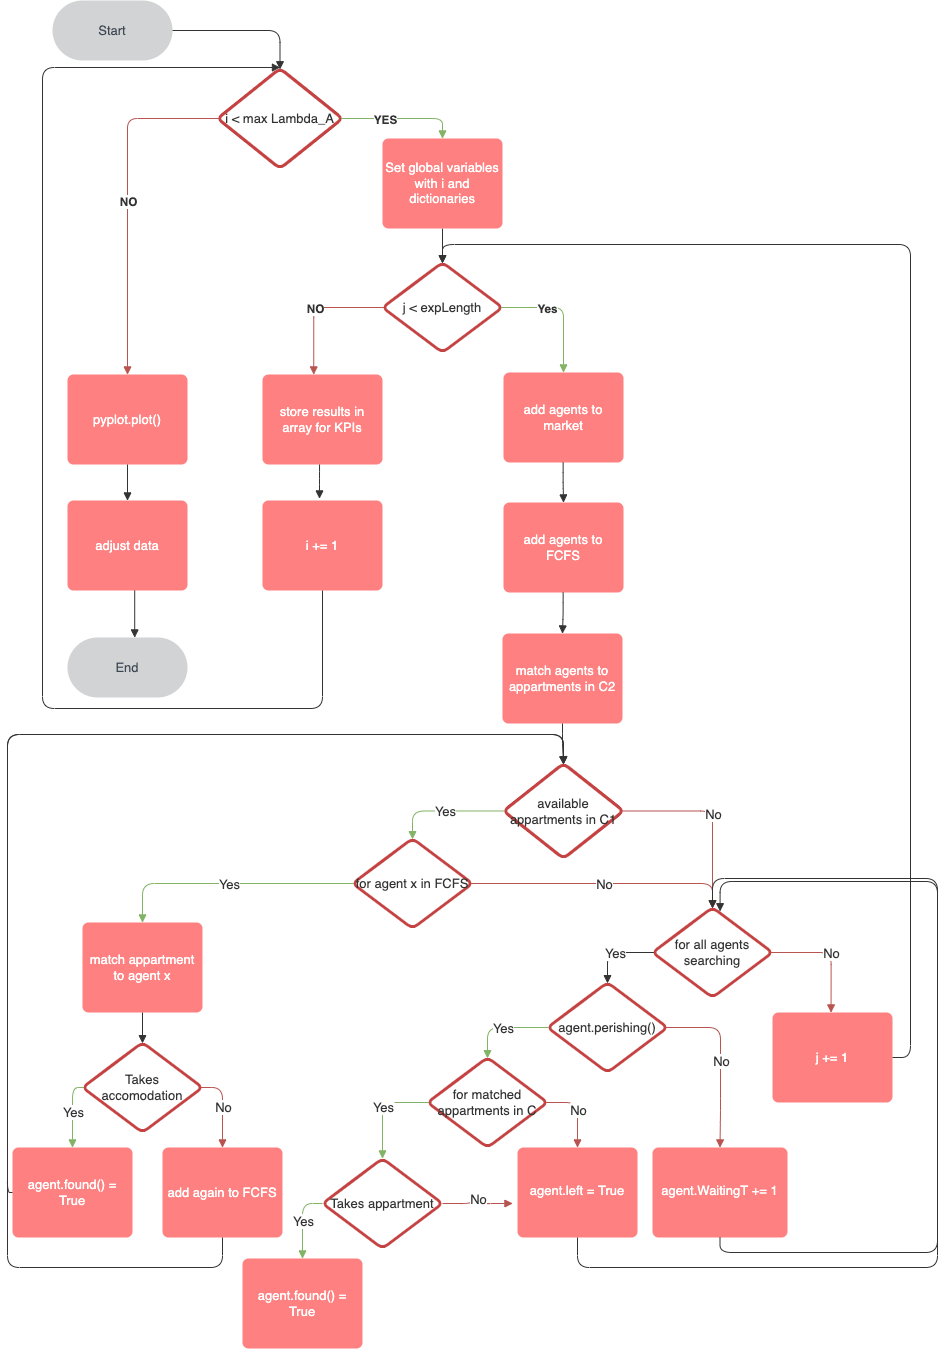
\includegraphics[width=0.71\linewidth]{figures/Flowchart.png}
\caption{The picture above encloses the code exposed in this chapter as a flowchart.}
\end{figure}

	\chapter{Experiment}

In this chapter we will discuss the simulations, the gathered data as well as the results. We will divide the chapter into three parts. In the first one we will make changes in the demand side of the model, in the second part we will alter the supply side and lastly we will compare the results and discuss about the results.

As previously mentioned in the past chapter we implemented category C1 and C2. Thus we will divide the supply section into two parts. The first one will contain the simulations of C1 and the second one of C2. We will alter the variables of the mentioned categories one at a time, leaving the rest of the variables untouched. 

Before we can start simulating we have to empirically search for minimum number of iteration that the model has to make in order for the market (ratios and KPIs) to converge. We will set the expLength (in second main loop) to a large number an plot it until we achieve a minimum number. As shown in the figure bellow, with static variables, the smallest value for expLength is 1500 in order to be completely sure that it will converge for all other $\lambda$ and probabilities to be tested. Then we will run the plots over the variable that will be tested as x-axis and not time/iterations.

\begin{figure}
    \centering
    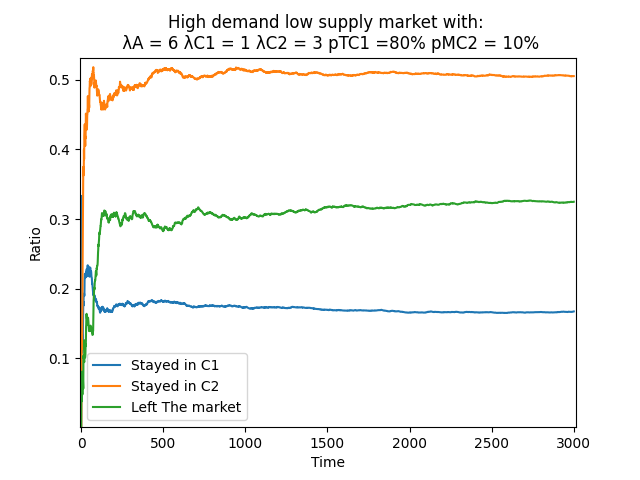
\includegraphics[width=0.6\linewidth]{figures/Rates_of_total_agents_distribution_over_time.png}
    \caption{Example of a market simulation with fixed variables over 3000 iterations with high demand and low supply converging.}
    \label{fig:convergence}
\end{figure}


\section{Changes in Demand}

In the demand side of the market there is one variables that can be changed. This variable being $\lambda$\A or the rate at which agents arrive to the market. In the next sections we will present market data while subject to changes in $\lambda$A.

\subsection{Simulations}

We will simulated the market with a wide range of values for $\lambda$A (0 to 20), going from a high supply and low demand in the early stages of the simulation and ending with very high demand and low supply. This with the purpose of demonstrating a shift of the market towards high demand and low supply Bellow we can find the data from the simulation for such a scenario. There is a graph for the mentioned KPIs as well as one for the average waiting times. For the extended results please refer to appendix \ref{fig:lATable} 


\begin{figure}
    \centering
    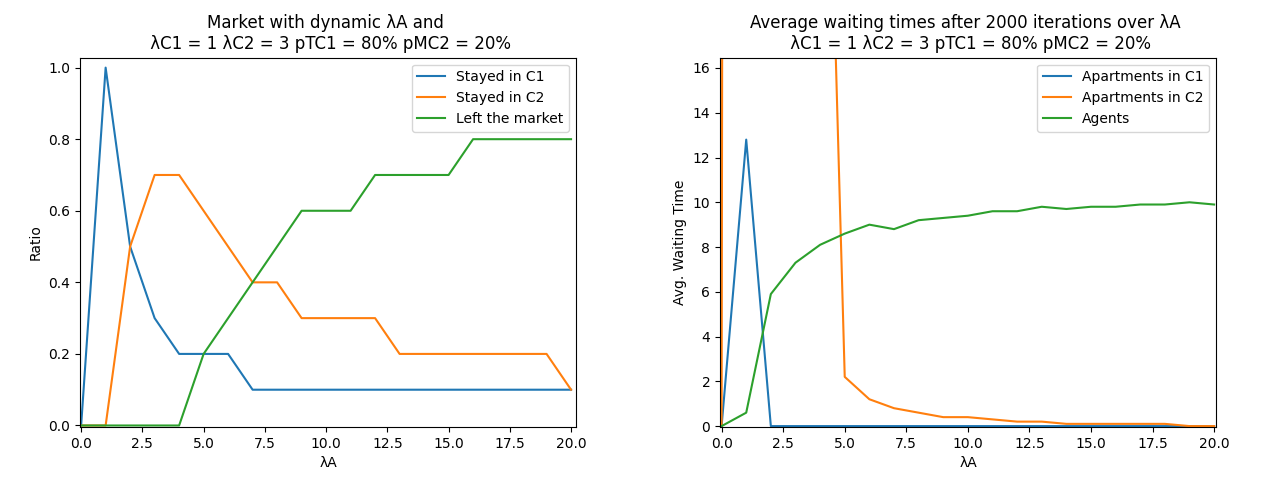
\includegraphics[width=1\linewidth, height = 7cm]{figures/lambdaA.png}
    \caption{Left: KPIs for changes in $\lambda$A. Right: Average waiting times of apartments in C1, C2 and the agents over changes in $\lambda$A.}
    \label{fig:KPIslambdaA}
\end{figure}

\subsection{Observations}

From \ref{fig:KPIslambdaA} we can see that the ratio of agents that left the market grow towards 1 and the ratio of agents that found some kind of accommodation (either in C1 or C2) falls towards 0. This is very straight forward since the supply never grows but the demand grows at a constant rate. At some point almost 100\% of the agents that arrive will not have the chance of finding accommodation an leave the market. Therefore we can assume that by running $\lambda$A towards infinity the ratio of agents that left/found will converge against 0 or 1 respectively.

The average waiting times from \ref{fig:KPIslambdaA} demonstrates that the more agents arrive to the market the higher the waiting time to find accommodation it gets. It eventually converges against 10, which is the average maximum waiting time assigned to them via the exponential distribution. This means they will eventually wait all the time then have since there is no accommodation possible and will leave the market. From the other side, the apartments waiting times converge against zero, since there is a point with too much demand but the demand stays constant. We can also observe that the waiting time of the houses starts at a high average and ends with zero. This is because in the beginning there are not enough agents to take all houses and thus are never occupied. We can also see that the spike in C1 is considerably smaller and falls at a faster rate than the one in C2. This is because agents prefer the C1 for its higher utility than C2.

We can see from these two figures that there is an equilibrium in the market. This is point is reached, when the sum of the agents equals the sum of apartments. In this precise example when $\lambda$A is equal to four. Here the ratio at which new apartments arrive to the market is the same as the ratio at which agents arrive. We can use this equilibrium to model the desired market. In this case we simulate with focus in a market with $\lambda A \geq 4$. 


\section{Changes in Supply}

The supply side of the model offers a wider variety of variables to manipulate. As mentioned we divided the next section into changes in C1 and C2. In category 1 we can change $\lambda$C1 that regulate the arrival of the new apartments to the market in C1 as well as \textbf{pTC1} that depicts the probability of the agent to take a matched accommodation in C1. For category 2 we can alter the variable $\lambda$C2 that is analogous to the one in category C1 and \textbf{pMC2} that computes the probability of the agent of being matched to an apartment. Note that in C1 there is no patching probability since it depends on the FCFS queue and in C2 there is no taking probability yet since C3 isn't implemented and there is no real decision to be made here.

\subsection{Changes in C1}

In this section we will present simulations of the market by changing the values $\lambda$C1 and \textbf{pTC1} but leaving the rest static. We will be altering the supply of apartments in C1 while leaving the arrivals of agents in the market and apartments in C2 constant.

\subsubsection{Simulations}

We ran the first simulation over $\lambda$C1 from 0 to 20 and plotted first over the KPIs ans then over the average waiting times. The table with the raw data for these plots can be found in the appendices of this paper. 

\begin{figure}
    \centering
    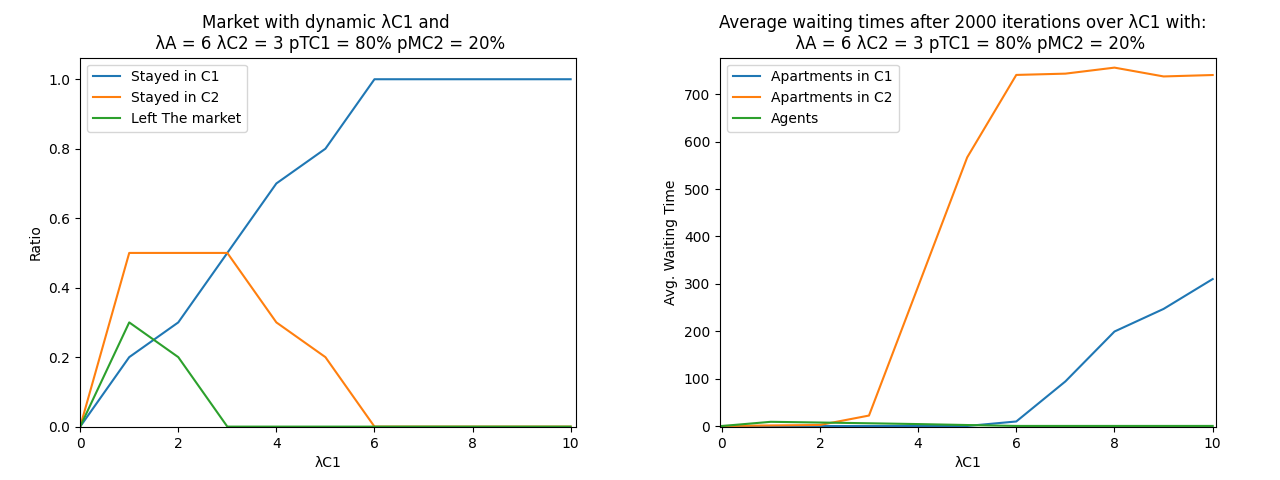
\includegraphics[width=1\linewidth, height = 7cm]{figures/lambdaC1inC1.png}
    \caption{Left: KPIs for changes in $\lambda$C1. Right: Average waiting times of apartments in C1, C2 and the agents over changes in $\lambda$C1.}
    \label{fig:c1lambdac1}
\end{figure}

Then we ran a second simulation with \textbf{pTC1} from 0 to 10 and changed the static variables since the effect of \textbf{pTC1} over C1 is better seen in a market with a more balanced demand-supply chain. We also made the intervals between data points smaller. They were increased by 0.5 instead of 1. This way we can simulate a short interval with more detail. To see the extended results please refer to \ref{fig:l1c1table} and \ref{fig:ptc1table}

\begin{figure}
    \centering
    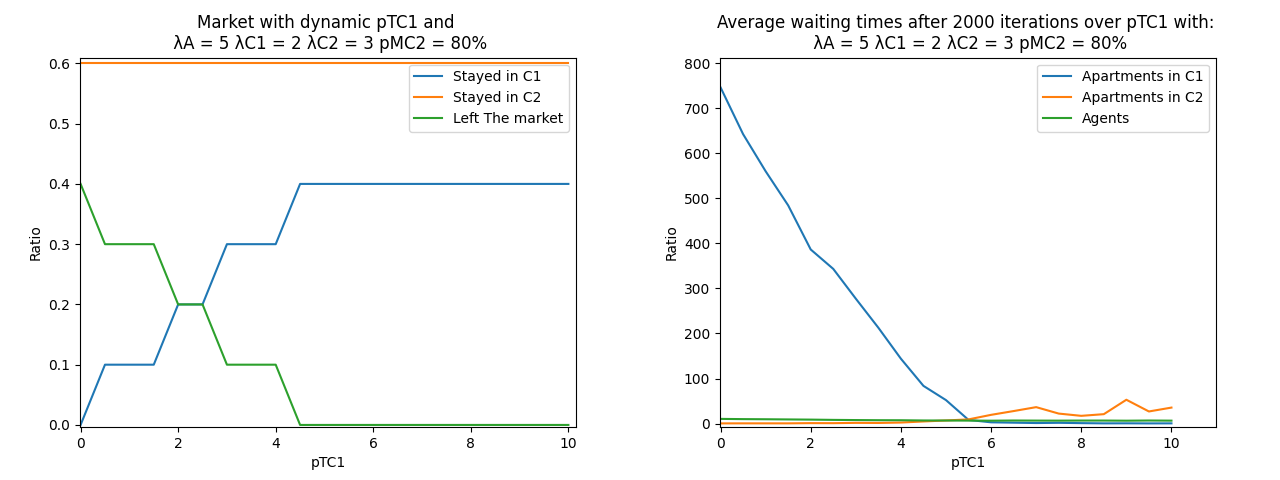
\includegraphics[width=1\linewidth, height = 7cm]{figures/pTC1.png}
    \caption{Left: KPIs for changes in \textbf{pTC1}. Right: Average waiting times of apartments in C1, C2 and the agents over changes in \textbf{pTC1}.}
    \label{fig:pTC1}
\end{figure}

\subsubsection{Observations}

From the simulations over $\lambda$C1 in figure \ref{fig:c1lambdac1} we can clearly observe, that the agents will always prefer C1 over C2. We can see that from interval 1 to 3 C2 has reaches its maximum since it is covering the supply in the market by its own with little apartments in C1. When  $\lambda$C1 takes the value of 3 the market hits its equilibrium point and C1 and C3 are equal. Here it is also important to remark, that from this point onwards no more agents have the necessity to leave the market. Afterwards C1 keeps taking demand away from C2 until all apartments in C2 are empty and all apartments from C1 are taken. Another example is how after the equilibrium point, the waiting times of C2 increase constantly while waiting times of C1 stay at zero just until the supply is greater than the demand when $\lambda$C1 is equal to 6.

Moreover we observed that for very low \textbf{pTC1} the waiting times of C1 increases considerably \ref{fig:pTC1}. However if we let this variable run we can see that the average waiting time of C1 rapidly decreases and when it hits 6\% it is already close to zero. This is because even though the probability of taking the apartment is very low, the agents will still prioritize accommodation in C1 and will wait in the FCFS queue again. Furthermore we can see how the lower the probability it is the more agents leave the market until it is around 6\% then the market converges, 60\% of the agents stays in C2 and 40\% in C1.

\subsection{Changes in C2}

In this section we will observe the market by changing the variables that control the supply side of the market specifically them of C2. The variables at our reach for this simulations are $\lambda$C2 and \textbf{pMC2}. 

\subsubsection{Simulations}

In figure \ref{fig:lambdac2} we simulated over $\lambda$C2 with an interval from 0 to 6. We chose a small interval for This since the plot converged quickly. We left the rest of the variables fixed as in the previous simulations of C1 and Demand. For the average waiting times plot we cut the plot when $\lambda$C2 reached 4. This choice was made since the waiting time of the apartments in C2 grew quickly and eventually the line for agents would disappear from the visual field.

\begin{figure}
    \centering
    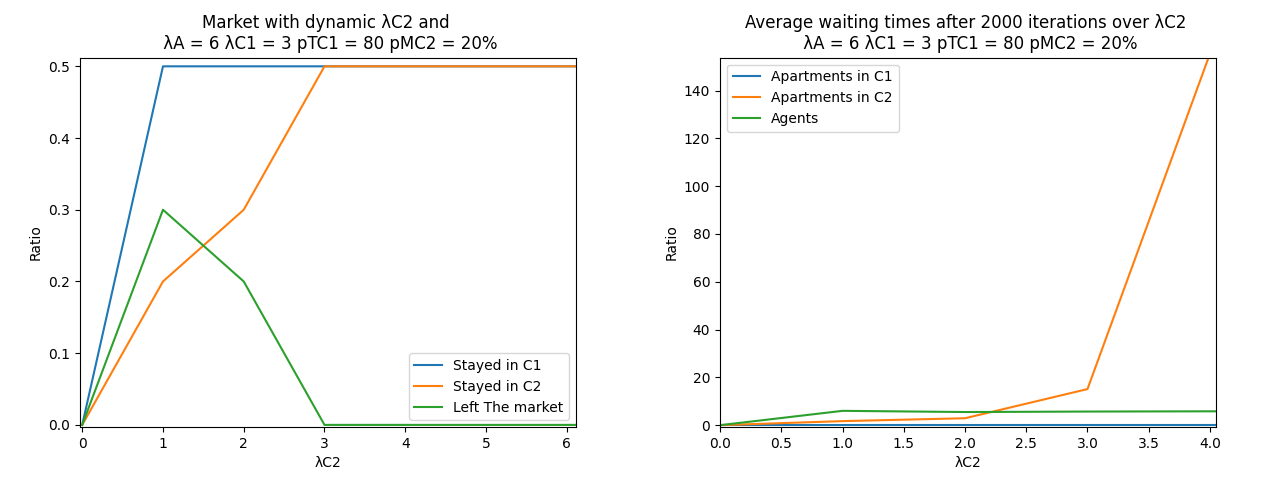
\includegraphics[width=1\linewidth, height = 7cm]{figures/lambdaC2.png}
    \caption{Left: KPIs for changes in $\lambda$C2. Right: Average waiting times of apartments in C1, C2 and the agents over changes in $\lambda$C2.}
    \label{fig:lambdac2}
\end{figure}

Then we plotted over the matching probability \textbf{pMC2} from 0 to 40. For this simulation we chose smaller lambdas since the simulation running time was very high and this shortened the running time considerably. Moreover with these new values for the fixed variables the effects of \textbf{pCM2} on the market are more pronounced. The extended results can be found in \ref{fig:lc2table} and \ref{fig:pmc2table}

\begin{figure}
    \centering
    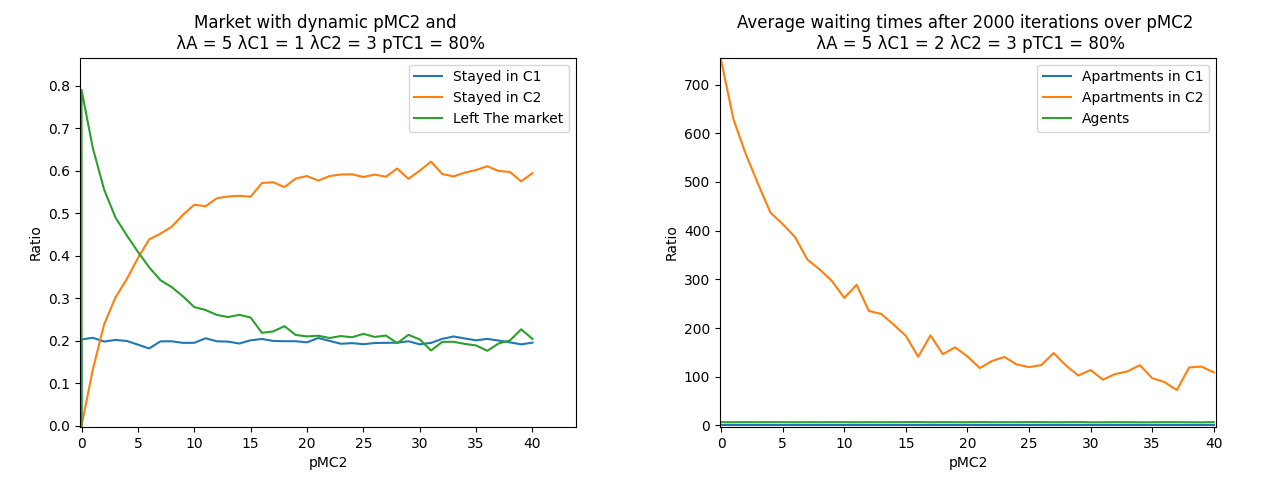
\includegraphics[width=1\linewidth, height = 7cm]{figures/pMC2.png}
    \caption{Left: KPIs for changes in \textbf{pMC2}. Right: Average waiting times of apartments in C1, C2 and the agents over changes in \textbf{pMC2}.}
    \label{fig:pMC2}
\end{figure}

\subsubsection{Observations}

From figure \ref{fig:lambdac2} we can observe, that over the whole period of time, the Houses in C1 where occupied, including when there were an over supply of accommodations in C2. Moreover the equilibrium point here is reached when $\lambda$C2 is equal to 3. At this point supply and demand are equal and the market is balances. Afterwards there are zero or close to zero agents leaving the market. For an agent to leave the market under these circumstances he would need to have spawned with a very low maximum time in order to not have had a chance in the FCFS queue and little time to be matched to apartments int C2. Furthermore, from the average waiting times we can see, that from the point where the market hits its equilibrium, any extra apartment in C2 will not be occupied and the waiting times will rise. We can also see that from  interval 2 to 3 the average waiting time of C2 is rising but not at the same rate after point 3. This is because even though there are more than enough houses to accommodate the whole demand of the market, the against will still prefer to wait for accommodation in C1 and waiting until the last opportunity to take something in C2.

Additionally we can see from figure \ref{fig:pMC2}, that in a balanced market (or a market in equilibrium) where demand equals the supply, if the matching probability for C2 is too low, many agents will not be able to find any accommodation. Moreover we can see that after crossing a probability of 30\% the market no longer reacts to this probability and it converges. This plot also relates directly to the average waiting times of the apartments in C2, where after the probability is 30\% the waiting time doesn't change much. On the other hand any matching probability lower than 30\% results in a higher waiting time of the houses in order to find an agent to accommodate. In order to see all the data please refer to the appendices of this paper where the data for all plots will be presented.

\section{Overall Data Analysis}

On this section we will discuss the results of the simulations presented in the section above. We will interpret and discuss the results. From the early observations we can see, that the market hits equilibrium points where the demand and supply can support each other. Moreover we saw that for an equilibrium point where the agents don't leave the market. The supply side hast to be lightly higher than the demand side when the taking and matching probability are low, thus leaving some apartments empty. On the other hand in order to have an equilibrium where all houses are taken and the supply and demand are exactly equal to each other, the take and match probability should be as close as possible to 100\%. This is an interesting phenomena and the explanation for that is that since the market is over saturated from the demand side, no matter if the probability is low since there are so many agents awaiting for accommodation that eventually one of them will take the place. Examples of these probabilities having to be very low in order to have an effect on the market are \ref{fig:pTC1} and \ref{fig:pMC2}. A big effect this probabilities are the waiting times, we observed that the lower the probability the higher the waiting times. This is because the agents have a smaller chance of taking\/matching to a certain apartment and if not they will wait more or go to the back of the FCFS queue.

Furthermore we saw that agents have strong preferences towards accommodations that offer a higher utility and they would even risk to have to leave the market in order to find accommodation in the public subsidised sector. We observed, that if it where possible the whole population of agents would stay in C1 replacing C2 entirely and at some point is no longer profitable to add more apartments in C2 since they will not be used. Figure \ref{fig:c1lambdac1} is a good example of that, as well as \ref{fig:lambdac2}.


Lastly we saw that we could divide all plots into three intervals and categorise them. From the supply side of the market, first we have the early stages of the plot where there is not enough apartments for the market and we observed agents leaving the market. Then we have a point where the market reaches its equilibrium and at the end leaving the variables to "infinity" the market converges (with all agents having accommodation) and the average waiting times of the apartments with low utility sky rockets. On the other hand the simulations of the demand side of the market can also be always divided into three parts. Firstly there are not enough agents to fulfill the needs of the supply side of the market, the waiting times of the apartments are very high and those of the agents very low. Then the equilibrium point is reached as in the simulations for the supply side and all agents are accommodated. Lastly the by letting the agents in the market converge against infinity we will see that almost all agents will leave the market and their waiting times rises, on the other hand all possible accommodations in C1 and C2 are met and the ratio of arrived agents to taken accommodation will converge to zero. On the next section we will discuss about the possible application this software could have and how could it be improved and expanded


	\chapter{Improvements, applications and conclusion}

Finally after developing the model for a housing market with a supply shortage we have come across some observations, conclusions and possible improvements as future work. On this chapter we will deepen into these ideas. We will start by proposing a set of possible improvements and lastly present our conclusions over the project.

\section{Improvements}

While implementing and running simulations of the model we noticed that the time needed in order to implement the complete model exceeded the time planned for this paper and we left the Category 3 out of the implementation. For this reason we will start this section by exposing how the category 3 could be added to the model as well as expanding the plotting capabilities in order to plot over two variables in three dimensions and lastly implementing a utility function for the agents to help with the choice making.

Moreover at the end of the project we realised that in order for the simulation to run faster we would need to find a solution since each one took around  one and two hours to run. For this we will mention a proposal to increase the efficiency of the code as wee as improving the quality of the code by sharing methods across data classes.

\subsection{Category 3}

As mentioned in chapter 3 we implemented the model with C1 and C2 and left C3 aside. However the expansion to include it is straight forward. Firstly we would recommend to initialize the arrivals to the market in the same way as for C1 and C2. After initializing it we would then store them in a dictionary "landlords\_C3" the same as for C1 and c2. The change is that the matching procedure differs from the two other categories. 

The principle for the matching is that the agents is desperate to find accommodation or is about to perish and needs to diversify the way he is searching for accommodation. After a certain percentage of its time has been used he will then apply for accommodation in C3. Then he will be matched to options with the probability \textbf{pMC3} and either take the accommodation with probability \textbf{pTC3} or make use of an utility function to make a decision. The first option can be implemented analogously as in C2 but with lower probabilities. Fro the second option the utility function would need to be implemented, more on the in the next section.

As shown an expansion to include C3 is very much possible and the model could be expanded in a fast manner. However it would make sense to expand the model not only with a new category but also with the utility function in order to have a more dynamic apartment allocation. We will explain this concept in more detail next.

\subsection{Utility function}

When including C3 to the model the number of options an agent has or could have to choose accommodation from increases. In order to help the agent make the best decision for him we could develop a function that computes the utility an agent has on taking an apartment. The function we propose is a two tuple function. It computes the utility having as input the time the agent has waited (or still has before perishing) and the price (or integer value) of the apartment U = f(t, price). The more time passes the more willing is the agent to enter a higher category. Then with the used of the already known probabilities the agents gets matched as usual but when making a decision of which accommodation to take not only will the "taking probability" be consulted but also the utility \textbf{U} the agent gents from said apartment.

Moreover since the decision of taking the apartment or even applying to a new category can be now expanded to include the utility, the distribution of supply can be better tailored to a the desired housing market that will be implemented. In order to implement the utility function we would only need to add an attribute price/value to the landlord dictionary and the function f(t,price). The first one is very easy to implement as it only requires to add the extra attribute and we propose that this value can also be computed with the help of a exponential distribution for each category as we did with the maximum waiting times of the agents. This way we can modify the values of the apartments independently and are able to simulate them as similar or different as the scenario requires. This will make the decisions of the agents easier/tougher as we require them to be.

\subsection{3-D Plotting}

After having ran several simulations and observed the data we encountered cases where running over two variables would have been beneficial. This is the case since some variables are heavily linked together and this link could be better visualized by running them together over a 3-D plot. We implemented four modules capable of this. One to run over $\lambda$C2 and \textbf{pMC2}, the second one runs over $\lambda$C2 and $\lambda$C1 and the last one over $\lambda$C1 and \textbf{pTC1}.

The principal problem with this type of plotting is the time it takes for each simulation to finish. The estimated finish time to run a simulation over $\lambda$C1 from 0-10 and \textbf{pTC1} from 0-30 was 27 hours. Until the code isn't optimized, multi -threaded or ran in a data center, three dimensional plotting is not realistic under this model and hardware. The code is available and can be found in the source code.

\subsection{Efficiency}

As already mentioned, the time constraint was one of the biggest challenges for this paper. So an issue of great importance, was the time spent during the simulations. As an example a simulation with $\lambda$A = 10, $\lambda$C1 = 5 and $\lambda$C2 while computing the probability of \textbf{pTC1} from 0 to 30\% takes around two and a half hours. The hardware was a 1,4 GHz Quad-Core Intel Core i5 as CPU a Intel Iris Plus as GPU and 16GB of RAM. While tracking the usage of the hardware it was clear that it was being used very inefficiently. At all times only one core was being used and the GPU was barely used.

Our proposal to improve efficiency is to make use of the multi-threading libraries available in python. The approach here would be to divide the first main loop between threads. Taking the example of the used hardware and simulating over \textbf{pTC1} from 0 to 30. We have 4 cores that can individually run independent from each other as well 31 independent values from each other. We would then assign each thread a part of the variables to be simulated. Then the different cores would be able to run the simulation no precise order and at the end of the simulation order the results and pass them to the plotting methods. As an example lets assume that we divide the variables as follows with four threads: Thread\_1 computes from 0-8, Thread\_2 from 9-16, Thread\_3 from 17-23 and Thread\_4 24-31. This way we could theoretically reduce the computing time with the same hardware to under one hour.

Lastly we could use more of the GPU by delegating small arithmetic calculations to it and not to the CPU. An example of an easy arithmetic calculations that can be parallelized are the calculations of probabilities \textbf{pTC1} and \textbf{pMC2}. These probabilities are computed several times per iteration and would shorten the running time of the simulation if implemented to be computed in the GPU.

\subsection{Code quality}

For the purpose of quick prototyping we concentrated mainly in the functional side of the code and left the code quality for future work. There are code blocks that could be shared between modules.Each module computes a certain variable, lambda or waiting time. For example the module lambdaC1.py and lambdaC2.py computes over said lambdas in their respective categories. They use similar code blocks but it is not shared between them. The idea could is to centralize certain code blocks so they can be shared, thus reducing the code length, complexity and repetitive code adjustments.

\section{Applications}
The developed software could be expanded and improved as explained in the section above and thus could be used to simulate or approximate the market distribution of houses as well as the behaviour and choices of agents. The model can be filled with data from the housing and registry office and approximate a market as close as possible. There are several sectors that recollect this type of data with different purposes. The variables they would have to fill are the ones explained in the introduction of this paper. For example a government may use this type of model using their data to fill the variables of the simulation in order to observe the behaviour of their market and thus launch incentives to housing categories of the market in order to get to an equilibrium point and achieve the best possible growing and accommodation rate for the city. Moreover they can stop agents from going to other cities by accommodating them in the categories that the simulations recommend.

Furthermore this model offers a open source platform for further research and development and thus the model can be expanded, changed or adapted in order to use it for other similar markets. Some examples of this kind of markets behaviours are: job hunting (where there are many applicant but little jobs), organ transplantation (with  FCFS queue and sometimes lotteries and matching) as well as school allocation for agents (bests schools receive higher number of applications). This markets consists of a supply-demand chain where the demand exceeds the supply and agents apply for a chance of getting somethings out of the supply side. Nevertheless by expanding this model we can achieve a higher accuracy by simulating the housing market with existing data.

\section{Conclusion}

This paper aimed to research the housing market under a supply shortage by composing a model where agents and houses arrive to the market with a poison process and then code and compute several simulations of said model. Based on said simulations under the adoption of the model we developed, it can be concluded that agents will have strong inclination towards choosing housing in C1. This leads to C2 houses to have a higher average waiting time until they find an agent and will be left out of the market. The results also indicate that all markets under this model can be divided in three and all simulations passed through an equilibrium point where supply fulfilled all agents needs for accommodation. In the case of a market with a supply shortage we have shown that the market can be modeled and we can test what would happen if there were more apartments in C1 or C2 or with less agents in the market in order to meet the equilibrium point. This proved to be relevant information for government institutions that have to make incentive choices in order to stop people from leaving their territory because of lack of supply. This simulations bring a new overview and could potentially help to make more accurate decisions and incentives the places in supply that need help.


Lastly by providing an open source base code, model and documentation that can be easily expanded and molded to the user needs, we enabled further research in this sector. The code can be tailored to the needs of the user and could potentially even be molded to simulate other markets with this approach. With this and the achieved data result the paper achieved its purpose of making the housing market with supply shortage easier to visualize, understand and propose possible solutions for it.
\end{spacing}
\newpage
\thispagestyle{empty}
\null

\newpage
\addcontentsline{toc}{chapter}{List of figures}
\listoffigures

\newpage
\addcontentsline{toc}{chapter}{Appendix}
\appendix
\chapter{Extended Results}

\textbf{\begin{figure}
    \centering
    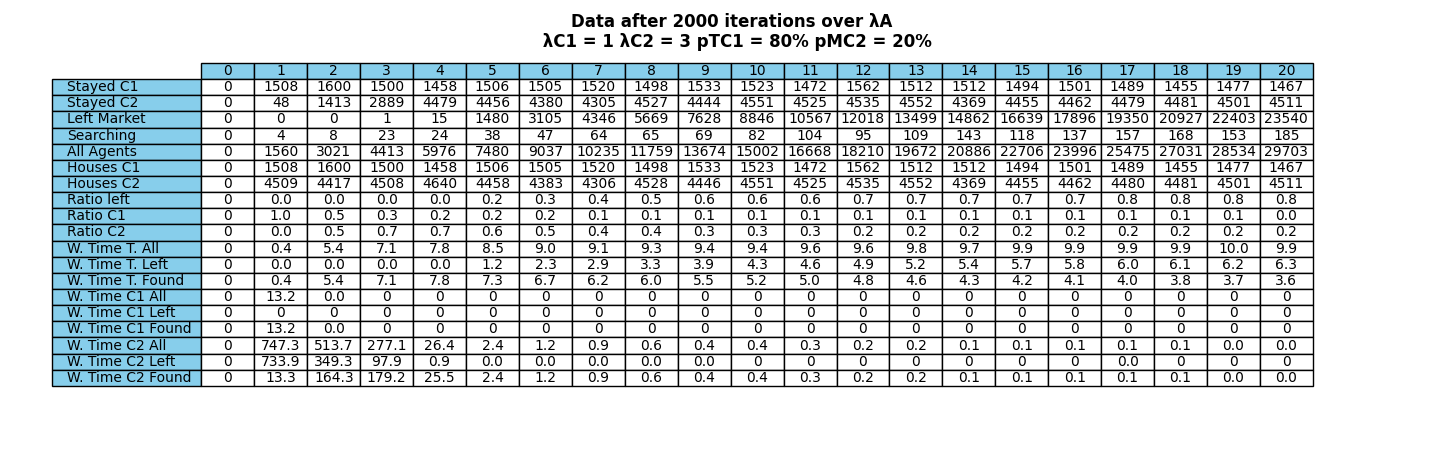
\includegraphics[width = 1\linewidth]{figures/lATable.png}
    \caption{Data table for simulations over $\lambda$A.}
    \label{fig:lATable}
\end{figure}}
\begin{figure}
    \centering
    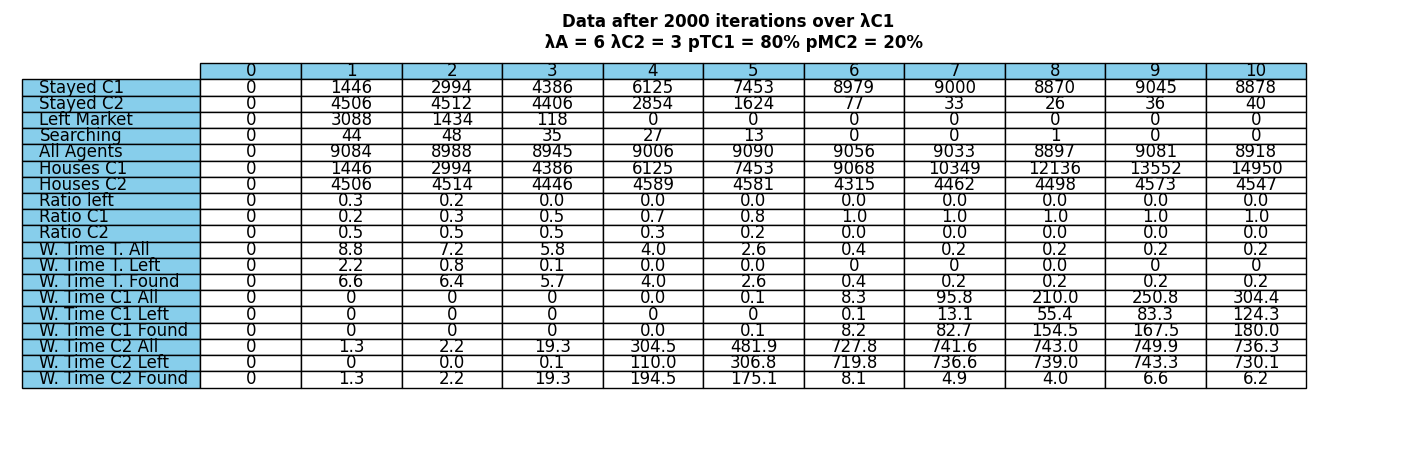
\includegraphics[width = 1\linewidth]{figures/lC1table.png}
    \caption{Data table for simulations over $\lambda$C1.}
    \label{fig:l1c1table}
\end{figure}
\begin{figure}
    \centering
    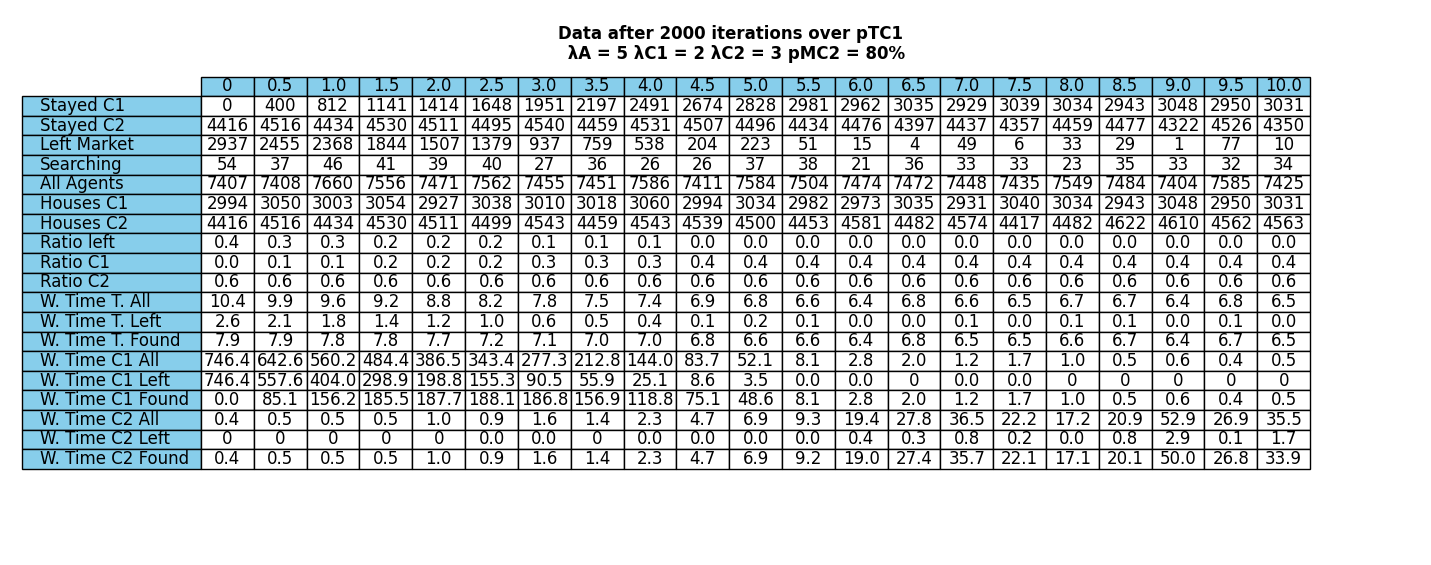
\includegraphics[width = 1\linewidth]{figures/ptC1Table.png}
    \caption{Data table for simulations over \textbf{pTC1}.}
    \label{fig:ptc1table}
\end{figure}
\begin{figure}
    \centering
    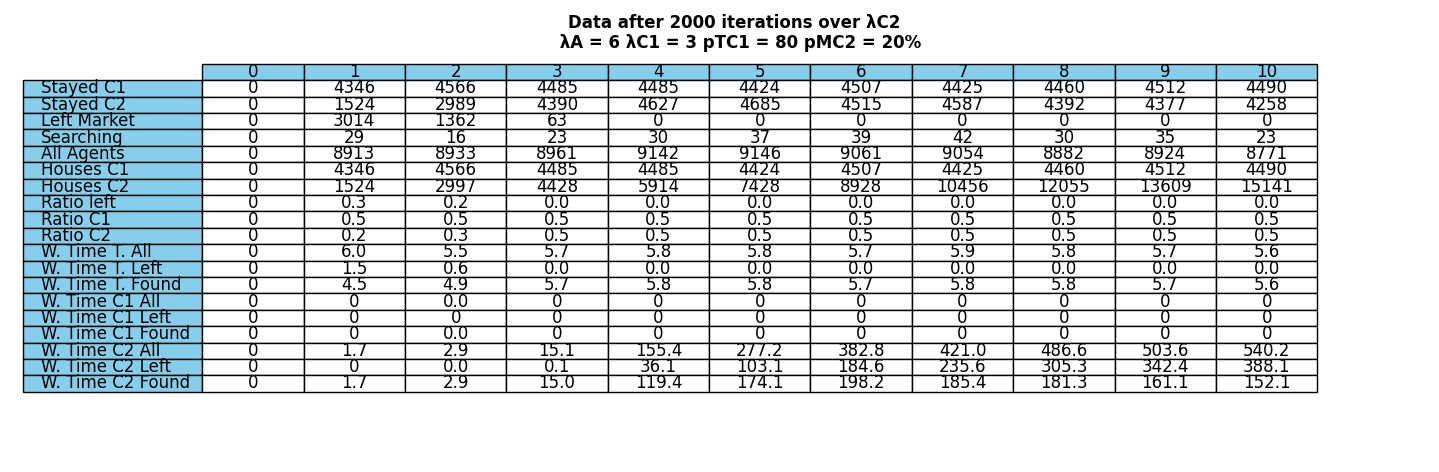
\includegraphics[width = 1\linewidth]{figures/pMC2table.png}
    \caption{Data table for simulations over $\lambda$C2.}
    \label{fig:lc2table}
\end{figure}
\begin{figure}
    \centering
    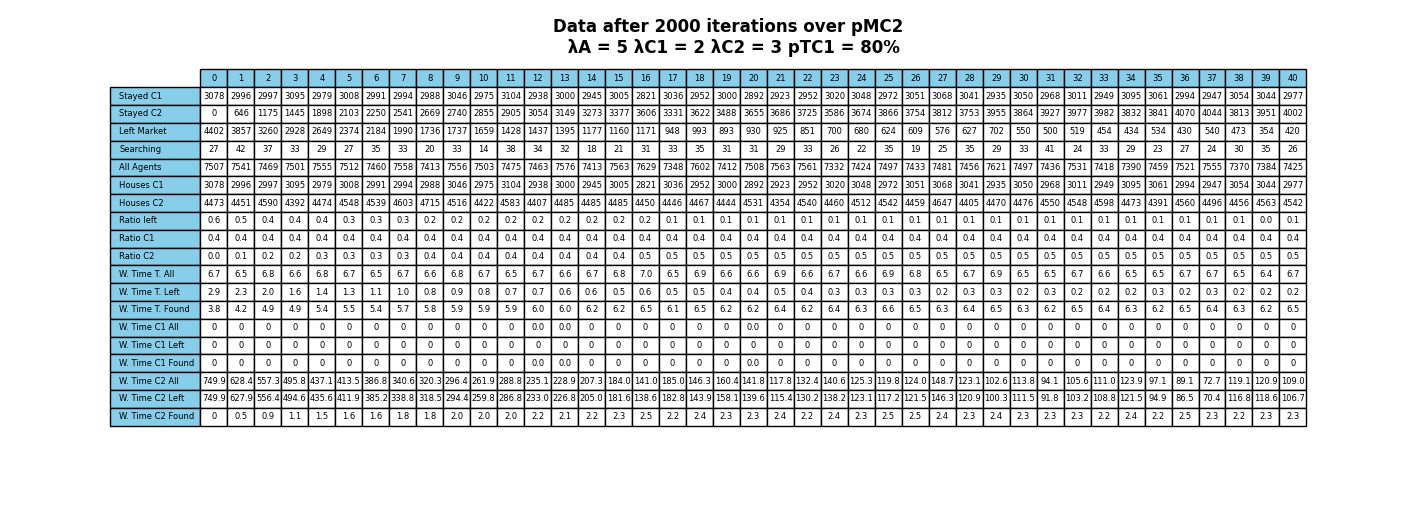
\includegraphics[width = 1\linewidth]{figures/lC2Table.png}
    \caption{Data table for simulations over \textbf{pMC2}.}
    \label{fig:pmc2table}
\end{figure}

\thispagestyle{empty}
\null
	
% Generierung des Literaturverzeichnisses
\newpage
\addcontentsline{toc}{chapter}{Bibliography}
\bibliography{citations.bib}

\end{document}
